En las etapas anteriores correspondientes al diseño se configuró y probó cada módulo, verificando su funcionamiento individual con el microcontrolador. Por lo que en esta sección se realizaron pruebas para verificar el funcionamiento de todos los módulos del sistema embebido y la aplicación móvil. \\

En la figura \ref{fig:integracion} se muestra la conexión del sensor de pulso, el sensor de temperatura y el módulo de comunicación con el microcontrolador, utilizando las conexiones proveídas por la tarjeta empleada durante este trabajo. \\

\begin{figure}[htbp!]
	\centering
	\fbox{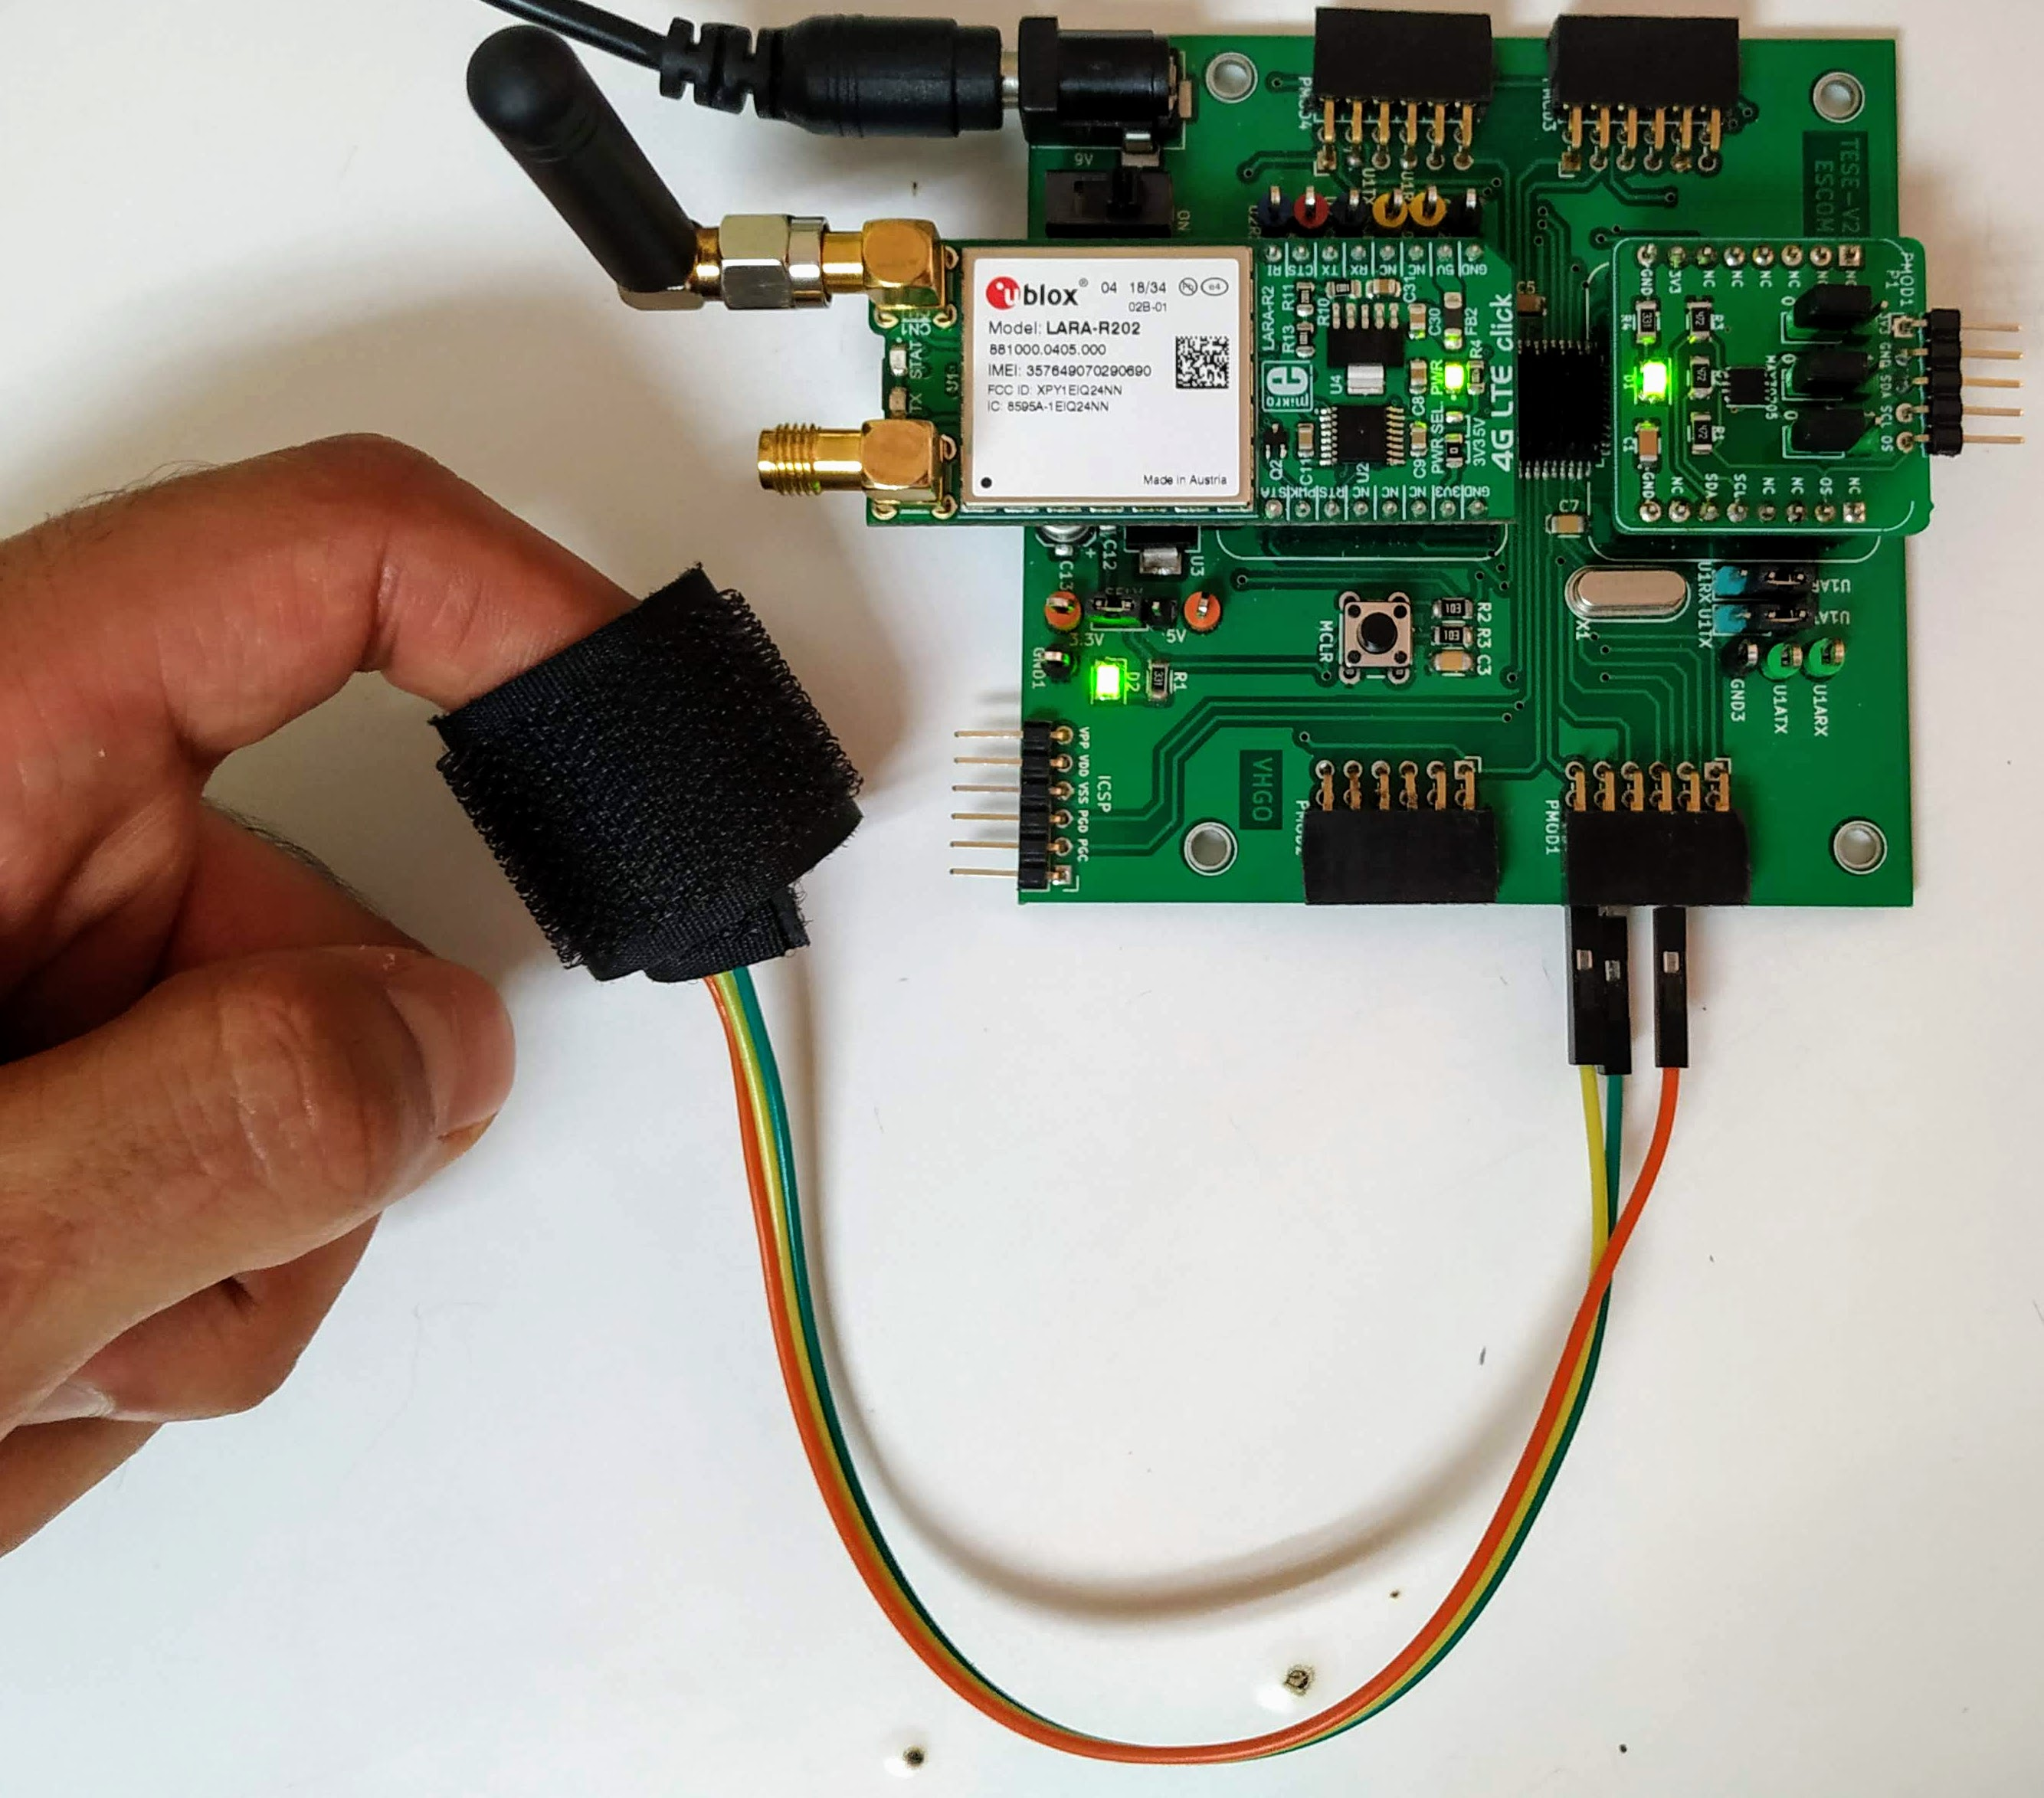
\includegraphics[width=0.6\textwidth]{AvancesPruebas/imagenes/integracion.jpg}}
	\caption{Sistema embebido.}
	\label{fig:integracion}
\end{figure}

Se enviaron mensajes de prueba para verificar que se respetaran las condiciones de envío del mensaje de texto y que el mensaje fuera recibido por el teléfono celular. Posteriormente se utilizó la aplicación móvil para el registro de un paciente y se verificó que se obtuviera la información de las mediciones contenidas en el mensaje, de manera automática desde la aplicación. \\

Durante este proceso se midió el tiempo de ejecución de las funciones del sistema embebido y se representó en una línea de tiempo mostrada en la figura \ref{fig:tiempoSistemaEmbebido}. Siendo el menor tiempo posible para el envío del mensaje de texto de 27 segundos a partir de iniciar la toma de medición de los signos vitales de un paciente.

\begin{figure}[htbp!]
	\centering
	\fbox{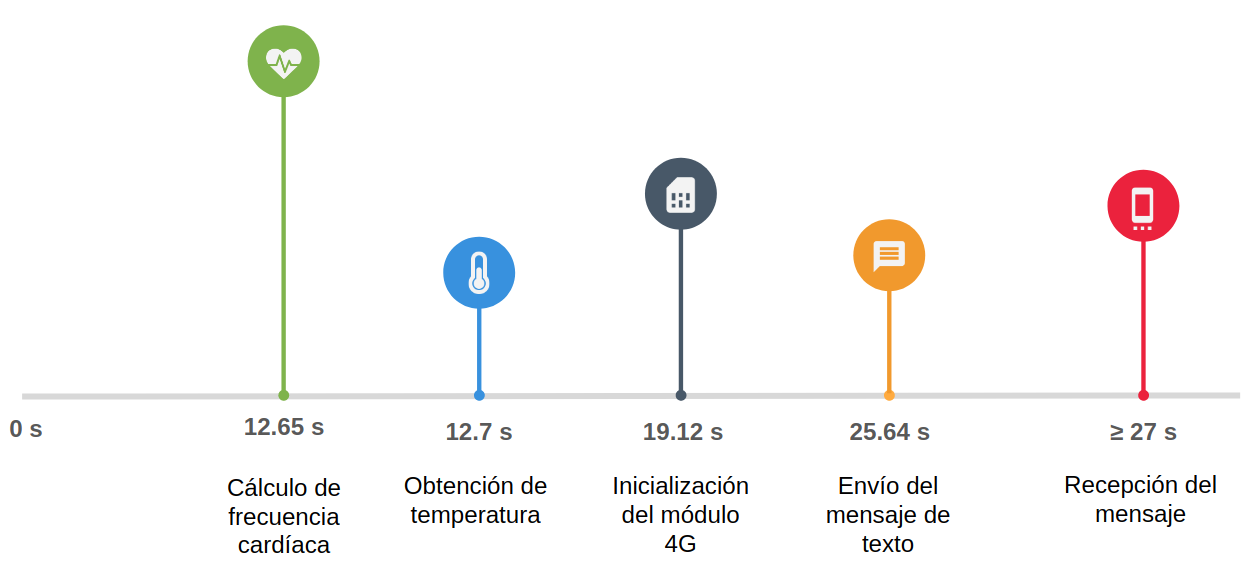
\includegraphics[width=1\textwidth]{AvancesPruebas/imagenes/tiempo.png}}
	\caption{Tiempo de ejecución del sistema embebido.}
	\label{fig:tiempoSistemaEmbebido}
\end{figure}
